%%%%%%%%%%%%%%%%%%%%%%%%%%%%%%%%%%%%%%%%%
% Short Sectioned Assignment LaTeX Template Version 1.0 (5/5/12)
% This template has been downloaded from: http://www.LaTeXTemplates.com
% Original author:  Frits Wenneker (http://www.howtotex.com)
% License: CC BY-NC-SA 3.0 (http://creativecommons.org/licenses/by-nc-sa/3.0/)
%%%%%%%%%%%%%%%%%%%%%%%%%%%%%%%%%%%%%%%%%

%----------------------------------------------------------------------------------------
%	PACKAGES AND OTHER DOCUMENT CONFIGURATIONS
%----------------------------------------------------------------------------------------

\documentclass[paper=a4, fontsize=11pt]{scrartcl} % A4 paper and 11pt font size

% ---- Entrada y salida de texto -----

\usepackage[T1]{fontenc} % Use 8-bit encoding that has 256 glyphs
\usepackage[utf8]{inputenc}
%\usepackage{fourier} % Use the Adobe Utopia font for the document - comment this line to return to the LaTeX default

% ---- Idioma --------
\usepackage[spanish]{babel}
%\usepackage[spanish]{babel} % Selecciona el español para palabras introducidas automáticamente, p.ej. "septiembre" en la fecha y especifica que se use la palabra Tabla en vez de Cuadro

% ---- Otros paquetes ----

\usepackage{url} % ,href} %para incluir URLs e hipervínculos dentro del texto (aunque hay que instalar href)
\usepackage{amsmath,amsfonts,amsthm} % Math packages
%\usepackage{graphics,graphicx, floatrow} %para incluir imágenes y notas en las imágenes
\usepackage{graphics,graphicx, float} %para incluir imágenes y colocarlas

% Para hacer tablas comlejas
%\usepackage{multirow}
%\usepackage{threeparttable}

%\usepackage{sectsty} % Allows customizing section commands
%\allsectionsfont{\centering \normalfont\scshape} % Make all sections centered, the default font and small caps

\usepackage{fancyhdr} % Custom headers and footers
\pagestyle{fancyplain} % Makes all pages in the document conform to the custom headers and footers
\fancyhead{} % No page header - if you want one, create it in the same way as the footers below
\fancyfoot[L]{} % Empty left footer
\fancyfoot[C]{} % Empty center footer
\fancyfoot[R]{\thepage} % Page numbering for right footer
\renewcommand{\headrulewidth}{0pt} % Remove header underlines
\renewcommand{\footrulewidth}{0pt} % Remove footer underlines
\setlength{\headheight}{13.6pt} % Customize the height of the header

\numberwithin{equation}{section} % Number equations within sections (i.e. 1.1, 1.2, 2.1, 2.2 instead of 1, 2, 3, 4)
\numberwithin{figure}{section} % Number figures within sections (i.e. 1.1, 1.2, 2.1, 2.2 instead of 1, 2, 3, 4)
\numberwithin{table}{section} % Number tables within sections (i.e. 1.1, 1.2, 2.1, 2.2 instead of 1, 2, 3, 4)

\setlength\parindent{0pt} % Removes all indentation from paragraphs - comment this line for an assignment with lots of text

\newcommand{\horrule}[1]{\rule{\linewidth}{#1}} % Create horizontal rule command with 1 argument of height

\graphicspath{ {./images/} }
\usepackage{subcaption}
\usepackage{hyperref}
\usepackage{soul}


%----------------------------------------------------------------------------------------
%	TÍTULO Y DATOS DEL ALUMNO
%----------------------------------------------------------------------------------------

\title{	
\normalfont \normalsize 
\textsc{\textbf{Series Temporales y Minería de Flujos de Datos (2019-2020)} \\ Máster Oficial Universitario en Ciencia de Datos e Ingeniería de Computadores \\ Universidad de Granada} \\ [25pt] % Your university, school and/or department name(s)
\horrule{0.5pt} \\[0.4cm] % Thin top horizontal rule
\huge Minería de Flujos de Datos. Trabajo Autónomo \\ % The assignment title
\horrule{2pt} \\[0.5cm] % Thick bottom horizontal rule
}

\author{Luis Balderas Ruiz \\ \texttt{DNI:77145416N. luisbalderas@correo.ugr.es}} 
 % Nombre y apellidos 


\date{\normalsize\today} % Incluye la fecha actual

%----------------------------------------------------------------------------------------
% DOCUMENTO
%----------------------------------------------------------------------------------------

\begin{document}

\maketitle % Muestra el Título

\newpage %inserta un salto de página

\tableofcontents % para generar el índice de contenidos

\listoffigures

\listoftables

\newpage

%
%\begin{figure}[H] %con el [H] le obligamos a situar aquí la figura
%	\centering
%	\includegraphics[scale=0.6]{e1.png}  %el parámetro scale permite agrandar o achicar la imagen. En el nombre de archivo puede especificar directorios
%	\caption{Progresión de la imagen de E en cada iteración} 
%	\label{fig:e1}
%\end{figure}


\section{Teoría}

\subsection{Cuestionario}

\subsection{Problema de clasificación}

\subsection{Concept Drift}

\section{Prácticas}

\subsection{Entrenamiento offline y evaluación posterior}

\subsubsection{Entrenamiento de un clasificador HoeffdingTree estacionario con generador WaveFormGenerator y varias semillas en entrenamiento. HoeffdingTree adaptativo}

Para enfrentar este problema, escribo un pequeño script con la ejecución en línea de órdenes de las sentencias necesarias para evaluar y entrenar un clasificador HoeffdingTree estacionario en primer lugar, y luego un HoeffdingTree adaptativo. Se hacen 30 ejecuciones por cada experimento propuesto, variando la semilla de entrenamiento entre 4 y 34

\begin{figure}[H] %con el [H] le obligamos a situar aquí la figura
	\centering
	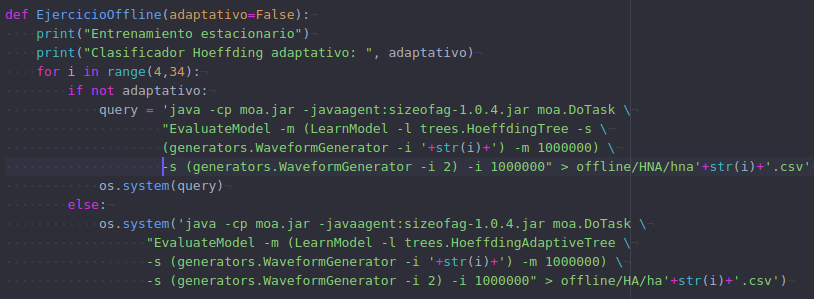
\includegraphics[scale=0.5]{off-code.png}  %el parámetro scale permite agrandar o achicar la imagen. En el nombre de archivo puede especificar directorios
	\caption{Código para la ejecución del Entrenamiento offline} 
	\label{fig:off1}
\end{figure}

Como resultado, al ejecutar la siguiente función, se genera un archivo que almacena los resultados de la precisión en clasificación y del estadístico Kappa:

\begin{figure}[H] %con el [H] le obligamos a situar aquí la figura
	\centering
	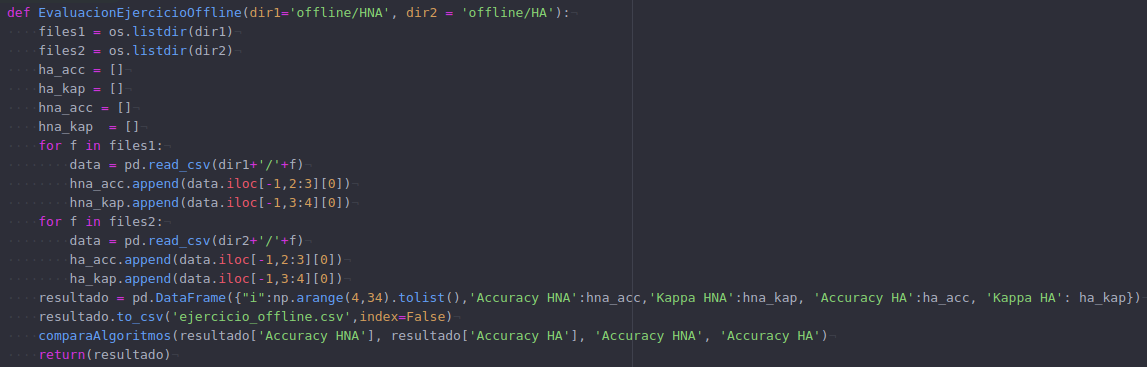
\includegraphics[scale=0.4]{off-ev.png}  %el parámetro scale permite agrandar o achicar la imagen. En el nombre de archivo puede especificar directorios
	\caption{Extracción de resultados en el Entrenamiento offline} 
	\label{fig:off2}
\end{figure}

dando lugar a la siguiente tabla de datos:
\begin{figure}[H] %con el [H] le obligamos a situar aquí la figura
	\centering
	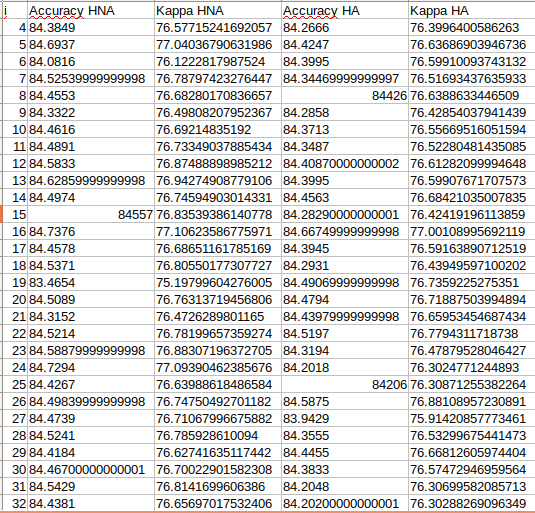
\includegraphics[scale=0.45]{ejercicio-offline.png}  %el parámetro scale permite agrandar o achicar la imagen. En el nombre de archivo puede especificar directorios
	\caption{Resultados de la precisión en clasificación y estadístico Kappa para Entrenamiento offline} 
	\label{fig:off3}
\end{figure}

\subsubsection{¿Cree que algún clasificador es significativamente mejor que el otro?}

A priori, revisando la tabla de resultados, no parece haber gran diferencia entre los dos clasificadores. Sin embargo, para asegurar la respuesta, es necesario aplicar una serie de test estadísticos: En primer lugar, el test de Shapiro-Wilk para comprobar la normalidad de las muestras, en este caso, de los resultados de la precisión. Si las muestras son normales, se aplica el test paramétrico t-test para ver si son significativamente distintas o no. Si no lo son, es necesario calcular la media de cada muestra para ver cuál es mayor. En el caso de no normalidad, debemos acudir a un test no paramétrico, como es el de Test U de Mann-Whitney para comprobar la diferencia entre las muestras. Si, siendo diferentes, alguna de ellas (o ambas) no siguen una distribución normal, calculamos la mediana en vez de la media para hacer la comparación. Para hacer todos estos cálculos, de aquí en adelante utilizo la siguiente función:

\begin{figure}[H] %con el [H] le obligamos a situar aquí la figura
	\centering
	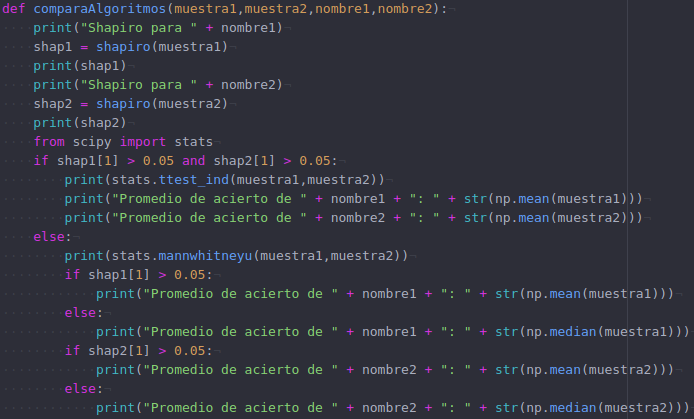
\includegraphics[scale=0.45]{comparaAl.png}  %el parámetro scale permite agrandar o achicar la imagen. En el nombre de archivo puede especificar directorios
	\caption{Método para comparar el rendimiento de dos algoritmos} 
	\label{fig:compAl}
\end{figure}

En concreto, para HoeffdingTree Adaptativo (HA) y HoeffdingTree no adaptativo (HNA), obtenemos que

\begin{figure}[H] %con el [H] le obligamos a situar aquí la figura
	\centering
	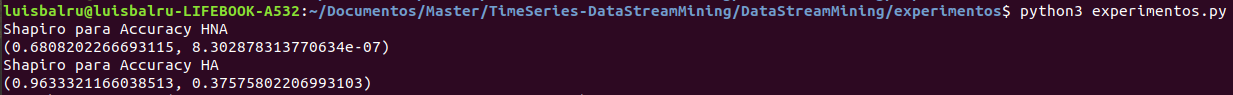
\includegraphics[scale=0.35]{off1.png}  %el parámetro scale permite agrandar o achicar la imagen. En el nombre de archivo puede especificar directorios
	\caption{Test de Shapiro-Wilk sobre HA y HNA} 
	\label{fig:off4}
\end{figure}
 
la población de resultados de precisión para el algoritmo Hoeffding Tree adaptativo sigue una distribución normal (p-valor 0.3757... > 0.05) a diferencia de Hoeffding Tree no adaptativo, (p-valor 8.3028...e-07 < 0.05, rechazando la hipótesis de normalidad). Por tanto, es necesario utilizar el test no paramétrico (ya que no se cumplen las hipótesis para los paramétricos) para comparar el rendimiento de los clasificadores. 

\begin{figure}[H] %con el [H] le obligamos a situar aquí la figura
	\centering
	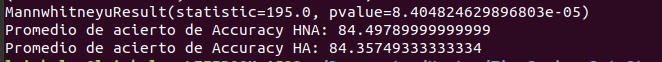
\includegraphics[scale=0.5]{off2.png}  %el parámetro scale permite agrandar o achicar la imagen. En el nombre de archivo puede especificar directorios
	\caption{Test U Mann Whitney y promedios para HA y HNA} 
	\label{fig:off5}
\end{figure}

Se obtiene un p-valor para el test de Mann-Whitney de 8.4048...e-05 < 0.05, por lo que se rechaza la hipótesis de que las distribuciones son iguales. Los promedios (HNA con mediana, HA con media) arrojan que el HNA es mejor que el HA, aunque la diferencia es bastante estrecha. 

\subsection{Entrenamiento online}

\subsubsection{Entrenamiento de un clasificador HoeffdingTree online (Interleaved Test-Then-Train) con generador WaveFormGenerator y varias semillas en entrenamiento. HoeffdingTree adaptativo}

En esta ocasión, ejecutamos un entrenamiento online con el método Interleaved Test-Then-Train y con generado WaveFormGenerator para los clasificadores HoeffdingTree y HoeffdingTree adaptativo. Para ello, hacemos 30 ejecuciones con semillas distintas para generar una población de resultados y comparar los resultados:

\begin{figure}[H] %con el [H] le obligamos a situar aquí la figura
	\centering
	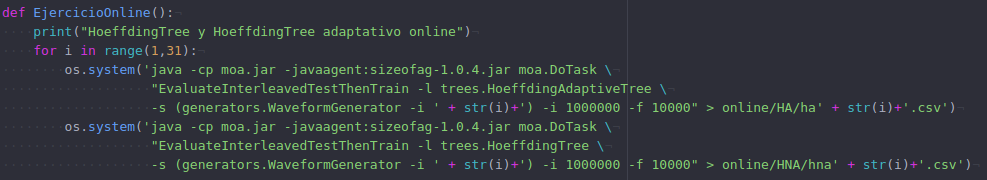
\includegraphics[scale=0.4]{onl1.png}  %el parámetro scale permite agrandar o achicar la imagen. En el nombre de archivo puede especificar directorios
	\caption{Entrenamiento online para HA y HNA} 
	\label{fig:onl1}
\end{figure}

Recogemos los resultados en la siguiente tabla:

\begin{figure}[H] %con el [H] le obligamos a situar aquí la figura
	\centering
	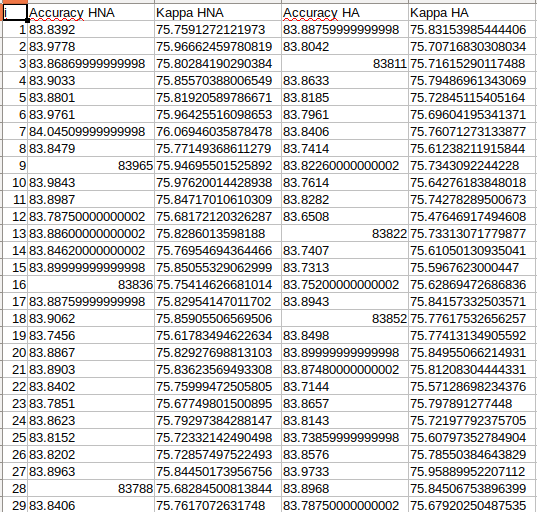
\includegraphics[scale=0.4]{onl-res.png}  %el parámetro scale permite agrandar o achicar la imagen. En el nombre de archivo puede especificar directorios
	\caption{Resultados del Entrenamiento online para HA y HNA} 
	\label{fig:onl2}
\end{figure}

\subsubsection{¿Cree que algún clasificador es significativamente mejor que el otro?}

De nuevo vemos que los resultados en accuracy son parejos, todos alrededor de un 83\%. Sin embargo, realizo un estudio más detenido basado en test estadísticos. Primero, para poder aplicar un test que compare las dos muestras, debemos comprobar si son normales o no a través del test de Shapiro-Wilk:

\begin{figure}[H] %con el [H] le obligamos a situar aquí la figura
	\centering
	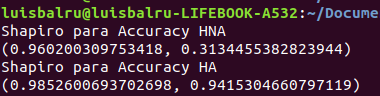
\includegraphics[scale=0.4]{onl3.png}  %el parámetro scale permite agrandar o achicar la imagen. En el nombre de archivo puede especificar directorios
	\caption{Shapiro-Wilk sobre Entrenamiento online para HA y HNA} 
	\label{fig:onl3}
\end{figure}

Como ambos p-valores son mayores que 0.05, no podemos rechazar la hipótesis de normalidad, luego la asumimos. Siendo así, es posible aplicar un test paramétrico, por lo que utilizo el t-test:

\begin{figure}[H] %con el [H] le obligamos a situar aquí la figura
	\centering
	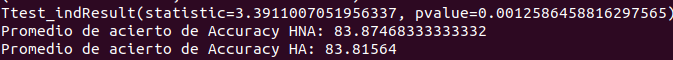
\includegraphics[scale=0.4]{onl4.png}  %el parámetro scale permite agrandar o achicar la imagen. En el nombre de archivo puede especificar directorios
	\caption{t-test y promedios para HA y HNA} 
	\label{fig:onl4}
\end{figure}

El p-valor del t-test es menor que 0.05, por lo que rechazamos la hipótesis de que las distribuciones sean iguales y, como ambas son normales, calculamos el promedio vía la media, obteniendo que HoeffdingTree Adaptativo tiene un mejor rendimiento.

\subsection{Entrenamiento online en datos con concept drift}

Para el entrenamiento online, sobre el método InterleavedTestThenTrain, con HoeffdingTree y la configuración indicada del generador RandomRBFGeneratorDrift, planteo la siguiente orden en la interfaz gráfica de MOA:

\textit{EvaluateInterleavedTestThenTrain -l trees.HoeffdingTree -s (generators.RandomRBFGeneratorDrift -s 0.001 -k 3 -a 7 -n 3) -i 2000000}

siendo s la velocidad de cambio de los centroides en el modelo, k el número de centroides con drift, a el número de atributos, n el número de centroides, c número de clases (por defecto 2), i la semilla para la generación de instancias y r la semilla para la generación del modelo (por defecto 1 ambas). En consecuencia, se obtienen los siguientes resultados, primero la gráfica de la precisión y luego los estadísticos:

\begin{figure}[H] %con el [H] le obligamos a situar aquí la figura
	\centering
	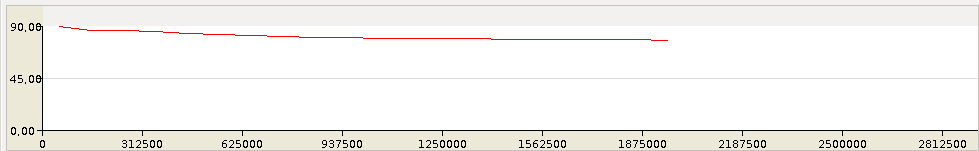
\includegraphics[scale=0.4]{cd1.png}  %el parámetro scale permite agrandar o achicar la imagen. En el nombre de archivo puede especificar directorios
	\caption{Gráfica de precisión en la clasificación respecto al número de instancias} 
	\label{fig:cd1}
\end{figure}

Vemos en la gráfica que el rendimiento va decayendo lentamente conforme aumenta el número de instancias. Si observamos los valores estadísticos

\begin{figure}[H] %con el [H] le obligamos a situar aquí la figura
	\centering
	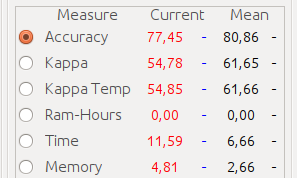
\includegraphics[scale=0.5]{cd2.png}  %el parámetro scale permite agrandar o achicar la imagen. En el nombre de archivo puede especificar directorios
	\caption{Medidas de rendimiento del modelo} 
	\label{fig:cd2}
\end{figure}

obtenemos un 80.86\% de accuracy y un Kappa de 61.65.

Pasamos ahora al clasificador HoeffdingTree adaptativo:

\textit{EvaluateInterleavedTestThenTrain -l trees.HoeffdingAdaptiveTree -s (generators.RandomRBFGeneratorDrift -s 0.001 -k 3 -a 7 -n 3) -i 2000000}

Presentamos a continuación los resultados de curva de acierto:

\begin{figure}[H] %con el [H] le obligamos a situar aquí la figura
	\centering
	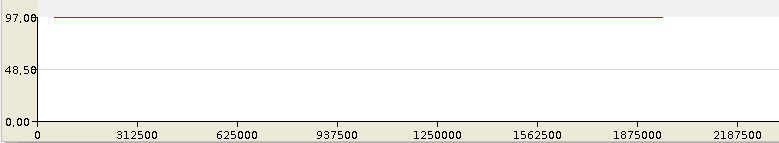
\includegraphics[scale=0.4]{cd3.png}  %el parámetro scale permite agrandar o achicar la imagen. En el nombre de archivo puede especificar directorios
	\caption{Gráfica de precisión en la clasificación respecto al número de instancias} 
	\label{fig:cd3}
\end{figure}

Si bien es cierto que los tests estadísticos en las secciones anteriores nos han indicado que se encontraban diferencias entre HoeffdingTree y HoeffdingAdaptiveTree, el rendimiento era prácticamente parejo. Podríamos extraer la idea de que, si no hay cambio de concepto, un clasificador y su versión adaptativa no tienen apenas diferencias. Esta es la primera vez en la que vemos la mejoría de la adaptación respecto del algoritmo original, habida cuenta de que este último iba empeorando su rendimiento conforme se introducían los nuevos datos y, sin embargo, el adaptativo obtiene un resultado estable y, además, muy bueno. Lo confirmamos con la tabla de medidas:

\begin{figure}[H] %con el [H] le obligamos a situar aquí la figura
	\centering
	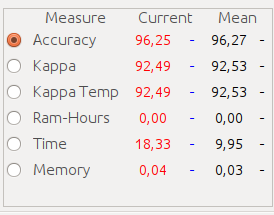
\includegraphics[scale=0.4]{cd4.png}  %el parámetro scale permite agrandar o achicar la imagen. En el nombre de archivo puede especificar directorios
	\caption{Medidas de rendimiento del algoritmo HoeffdingAdaptiveTree} 
	\label{fig:cd4}
\end{figure}

viendo que, verdaderamente, hay diferencias significativas. Lo confirmamos a continuación con un estudio estadístico, modificando las semillas.



\subsection{Entrenamiento online en datos con concept drift, incluyendo mecanismos para olvidar instancias pasadas}

\subsection{Entrenamiento online en datos con concept drift, incluyendo mecanismos para reiniciar modelos tras la detección de cambios de concepto}




\newpage
\section{Bibliografía}

%------------------------------------------------

\bibliography{citas} %archivo citas.bib que contiene las entradas 
\bibliographystyle{plain} % hay varias formas de citar

\end{document}
